\documentclass[12pt,a4paper]{article}
\usepackage[utf8]{inputenc}
\usepackage[T1]{fontenc}
\usepackage[english]{babel}
\usepackage{graphicx}
\usepackage{hyperref}
\usepackage{listings}
\usepackage{xcolor}
\usepackage{geometry}
\usepackage{fancyhdr}
\usepackage{titlesec}
\usepackage{booktabs}
\usepackage{longtable}
\usepackage{enumitem}
\usepackage{float}
\usepackage{caption}
\usepackage{subcaption}
\usepackage{amsmath}
\usepackage{tikz}
\usetikzlibrary{shapes,arrows,positioning}

\geometry{margin=2.5cm}

% Code listing style
\definecolor{codegreen}{rgb}{0,0.6,0}
\definecolor{codegray}{rgb}{0.5,0.5,0.5}
\definecolor{codepurple}{rgb}{0.58,0,0.82}
\definecolor{backcolour}{rgb}{0.95,0.95,0.92}

\lstdefinestyle{mystyle}{
    backgroundcolor=\color{backcolour},
    commentstyle=\color{codegreen},
    keywordstyle=\color{magenta},
    numberstyle=\tiny\color{codegray},
    stringstyle=\color{codepurple},
    basicstyle=\ttfamily\footnotesize,
    breakatwhitespace=false,
    breaklines=true,
    captionpos=b,
    keepspaces=true,
    numbers=left,
    numbersep=5pt,
    showspaces=false,
    showstringspaces=false,
    showtabs=false,
    tabsize=2,
    frame=single
}
\lstset{style=mystyle}

\pagestyle{fancy}
\fancyhf{}
\rhead{Assignment 3 - Energy Management System}
\lhead{Distributed Systems}
\rfoot{Page \thepage}

\begin{document}

% Title Page
\begin{titlepage}
    \centering
    \vspace*{2cm}
    
    {\Huge\bfseries Energy Management System\\[0.5cm]}
    {\LARGE Assignment 3\\[0.3cm]}
    {\Large Real-Time Communication \& Customer Support\\[2cm]}
    
    \includegraphics[width=0.3\textwidth]{placeholder-logo.png}\\[2cm]
    
    {\Large\bfseries Distributed Systems Course\\[0.5cm]}
    {\large Technical University\\[1cm]}
    
    \vfill
    
    {\large\bfseries Author:}\\
    Student Name\\[0.5cm]
    
    {\large\bfseries Date:}\\
    December 2025\\[1cm]
    
\end{titlepage}

\tableofcontents
\newpage

% ============================================
% SECTION 1: INTRODUCTION
% ============================================
\section{Introduction}

\subsection{Project Overview}
This document presents the implementation of Assignment 3 for the Energy Management System, focusing on real-time communication capabilities and intelligent customer support features.

\subsection{Objectives}
The main objectives of Assignment 3 are:
\begin{itemize}
    \item \textbf{WebSocket Microservice} - Real-time overconsumption notifications
    \item \textbf{Rule-Based Chatbot} - Customer support with 10+ rules
    \item \textbf{AI-Driven Support (Bonus)} - Google Gemini API integration
    \item \textbf{Client-to-Admin Chat (Bonus)} - Bidirectional real-time chat
\end{itemize}

\subsection{Technologies Used}
\begin{table}[H]
\centering
\begin{tabular}{|l|l|l|}
\hline
\textbf{Category} & \textbf{Technology} & \textbf{Purpose} \\
\hline
Backend & Spring Boot 3.1.5 & Microservices framework \\
WebSocket & Spring WebSocket & Real-time communication \\
Message Queue & RabbitMQ 3.13 & Async messaging \\
AI & Google Gemini API & Intelligent responses \\
Frontend & Next.js 14 & React framework \\
Styling & Tailwind CSS & UI styling \\
Container & Docker & Containerization \\
Proxy & Traefik & Reverse proxy \\
\hline
\end{tabular}
\caption{Technologies Stack}
\end{table}

% ============================================
% SECTION 2: ARCHITECTURE
% ============================================
\section{System Architecture}

\subsection{Microservices Overview}
The system consists of 8 microservices working together:

\begin{table}[H]
\centering
\begin{tabular}{|l|l|l|l|}
\hline
\textbf{Service} & \textbf{Port} & \textbf{Database} & \textbf{Description} \\
\hline
Auth MS & 8083 & MySQL (3309) & Authentication \& JWT \\
User MS & 8081 & MySQL (3307) & User management \\
Device MS & 8082 & MySQL (3308) & Device CRUD \\
Monitoring MS & 8084 & MySQL (3310) & Energy monitoring \\
\textbf{WebSocket MS} & \textbf{8085} & - & \textbf{Real-time notifications} \\
\textbf{Customer Support MS} & \textbf{8086} & MySQL (3307) & \textbf{Chatbot \& AI} \\
Frontend & 3000 & - & Next.js UI \\
Traefik & 80 & - & Reverse proxy \\
\hline
\end{tabular}
\caption{Microservices Architecture}
\end{table}

\subsection{Communication Flow}
\begin{figure}[H]
\centering
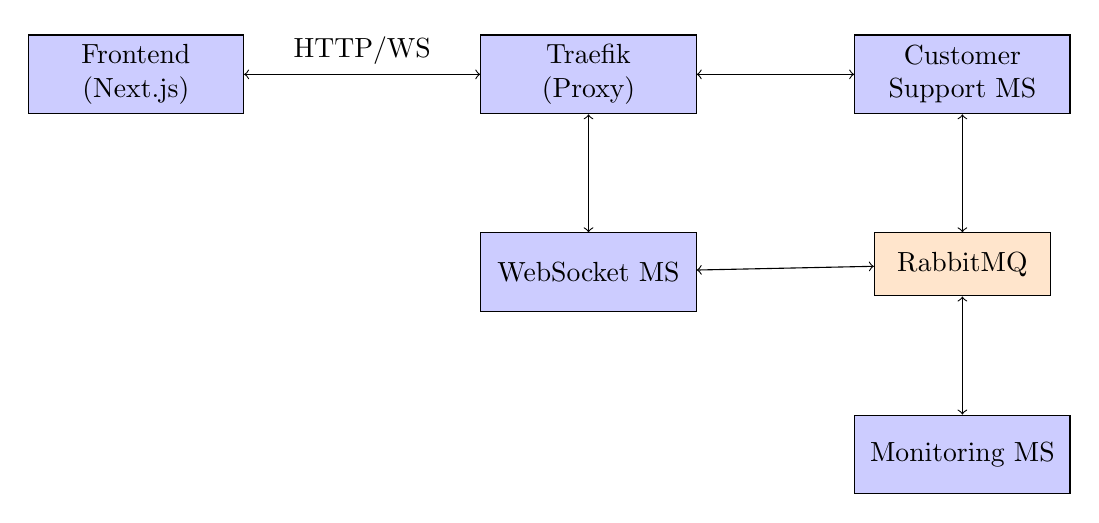
\begin{tikzpicture}[node distance=2cm, auto]
    % Styles
    \tikzstyle{service} = [rectangle, draw, fill=blue!20, text width=2.5cm, text centered, minimum height=1cm]
    \tikzstyle{queue} = [rectangle, draw, fill=orange!20, text width=2cm, text centered, minimum height=0.8cm]
    \tikzstyle{db} = [cylinder, draw, fill=green!20, shape border rotate=90, aspect=0.25, minimum height=1cm, minimum width=1.5cm]
    
    % Nodes
    \node[service] (frontend) {Frontend\\(Next.js)};
    \node[service, right=3cm of frontend] (traefik) {Traefik\\(Proxy)};
    \node[service, below=1.5cm of traefik] (websocket) {WebSocket MS};
    \node[service, right=2cm of traefik] (support) {Customer\\Support MS};
    \node[queue, below=1.5cm of support] (rabbitmq) {RabbitMQ};
    \node[service, below=1.5cm of rabbitmq] (monitoring) {Monitoring MS};
    
    % Arrows
    \draw[<->] (frontend) -- node[above] {HTTP/WS} (traefik);
    \draw[<->] (traefik) -- (websocket);
    \draw[<->] (traefik) -- (support);
    \draw[<->] (websocket) -- (rabbitmq);
    \draw[<->] (support) -- (rabbitmq);
    \draw[<->] (monitoring) -- (rabbitmq);
\end{tikzpicture}
\caption{System Communication Flow}
\end{figure}

% ============================================
% SECTION 3: PHASE 1 - WEBSOCKET MICROSERVICE
% ============================================
\section{Phase 1: WebSocket Microservice}

\subsection{Overview}
The WebSocket Microservice provides real-time notification capabilities for overconsumption alerts. When a device exceeds its maximum hourly consumption, users receive instant notifications.

\subsection{Project Structure}
\begin{lstlisting}[language=bash, caption=WebSocket Microservice Structure]
websocket-microservice/
├── src/main/java/com/energy/websocket/
│   ├── WebSocketApplication.java
│   ├── config/
│   │   ├── WebSocketConfig.java
│   │   └── RabbitMQConfig.java
│   ├── handler/
│   │   ├── NotificationWebSocketHandler.java
│   │   └── ChatWebSocketHandler.java
│   ├── listener/
│   │   ├── OverconsumptionListener.java
│   │   └── ChatMessageListener.java
│   └── dto/
│       ├── NotificationMessage.java
│       ├── OverconsumptionEvent.java
│       └── ChatMessage.java
├── pom.xml
└── Dockerfile
\end{lstlisting}

\subsection{WebSocket Configuration}
\begin{lstlisting}[language=Java, caption=WebSocketConfig.java]
@Configuration
@EnableWebSocket
@RequiredArgsConstructor
public class WebSocketConfig implements WebSocketConfigurer {
    
    private final NotificationWebSocketHandler notificationHandler;
    private final ChatWebSocketHandler chatHandler;
    
    @Override
    public void registerWebSocketHandlers(WebSocketHandlerRegistry registry) {
        registry.addHandler(notificationHandler, "/ws/notifications")
                .setAllowedOrigins("*");
        
        registry.addHandler(chatHandler, "/ws/chat")
                .setAllowedOrigins("*");
    }
}
\end{lstlisting}

\subsection{Overconsumption Flow}
\begin{enumerate}
    \item Device Simulator sends sensor data to RabbitMQ
    \item Monitoring MS aggregates hourly consumption
    \item If consumption exceeds max limit, publishes to \texttt{overconsumption\_queue}
    \item WebSocket MS receives event and broadcasts to connected clients
    \item Frontend displays toast notification
\end{enumerate}

\subsection{RabbitMQ Queues}
\begin{table}[H]
\centering
\begin{tabular}{|l|l|l|}
\hline
\textbf{Queue Name} & \textbf{Producer} & \textbf{Consumer} \\
\hline
sensor\_data\_queue & Device Simulator & Monitoring MS \\
overconsumption\_queue & Monitoring MS & WebSocket MS \\
chat\_queue & Customer Support MS & WebSocket MS \\
\hline
\end{tabular}
\caption{RabbitMQ Queue Configuration}
\end{table}

% ============================================
% SECTION 4: PHASE 2 - RULE-BASED CHATBOT
% ============================================
\section{Phase 2: Rule-Based Chatbot}

\subsection{Overview}
The Customer Support Microservice implements a rule-based chatbot with 11 predefined rules to handle common user queries automatically.

\subsection{Rule Interface}
\begin{lstlisting}[language=Java, caption=ChatRule Interface]
public interface ChatRule {
    boolean matches(String message);
    String getResponse(String message);
    int getPriority();
    String getRuleName();
}
\end{lstlisting}

\subsection{Implemented Rules}
\begin{longtable}{|l|l|p{6cm}|}
\hline
\textbf{Rule Name} & \textbf{Priority} & \textbf{Keywords} \\
\hline
\endhead
GreetingRule & 1 & hello, hi, hey, buna, salut \\
\hline
FarewellRule & 2 & bye, goodbye, thanks, thank you \\
\hline
HelpRule & 3 & help, how to, guide, tutorial \\
\hline
DeviceInfoRule & 10 & device, add device, create device \\
\hline
ConsumptionRule & 11 & consumption, energy, kwh, consum \\
\hline
OverconsumptionRule & 12 & overconsumption, exceeded, alert \\
\hline
AccountRule & 13 & account, profile, password, email \\
\hline
BillingRule & 14 & bill, payment, invoice, cost \\
\hline
TechnicalSupportRule & 15 & error, bug, not working, problem \\
\hline
DataExportRule & 16 & export, download, csv, report \\
\hline
MaxConsumptionRule & 17 & max consumption, limit, threshold \\
\hline
\caption{Implemented Chat Rules}
\end{longtable}

\subsection{Rule Processing Logic}
\begin{lstlisting}[language=Java, caption=RuleBasedChatService.java]
@Service
public class RuleBasedChatService {
    private final List<ChatRule> rules;
    private final GeminiService geminiService;
    
    public ChatResponse processMessage(String message) {
        // Sort rules by priority
        List<ChatRule> sortedRules = rules.stream()
            .sorted(Comparator.comparingInt(ChatRule::getPriority))
            .toList();
        
        // Try each rule
        for (ChatRule rule : sortedRules) {
            if (rule.matches(message)) {
                return ChatResponse.builder()
                    .response(rule.getResponse(message))
                    .isRuleBased(true)
                    .ruleName(rule.getRuleName())
                    .build();
            }
        }
        
        // Fallback to AI if no rule matches
        return geminiService.generateResponse(message);
    }
}
\end{lstlisting}

\subsection{API Endpoints}
\begin{table}[H]
\centering
\begin{tabular}{|l|l|p{5cm}|}
\hline
\textbf{Method} & \textbf{Endpoint} & \textbf{Description} \\
\hline
POST & /api/chat/message & Send message to chatbot \\
GET & /api/chat/rules & List all available rules \\
GET & /api/chat/health & Health check endpoint \\
POST & /api/chat/send & Send message to admin (bonus) \\
GET & /api/chat/history/\{userId\} & Get chat history (bonus) \\
\hline
\end{tabular}
\caption{Customer Support API Endpoints}
\end{table}

% ============================================
% SECTION 5: PHASE 3 - AI-DRIVEN SUPPORT (BONUS)
% ============================================
\section{Phase 3: AI-Driven Customer Support (Bonus +1p)}

\subsection{Overview}
When no rule matches the user's query, the system falls back to Google Gemini AI for intelligent responses. This provides a more natural conversation experience.

\subsection{Gemini API Integration}
\begin{lstlisting}[language=Java, caption=GeminiService.java]
@Service
public class GeminiService {
    private final WebClient webClient;
    
    @Value("${gemini.apiKey}")
    private String apiKey;
    
    public ChatResponse generateResponse(String userMessage) {
        String prompt = buildPrompt(userMessage);
        
        GeminiRequest request = GeminiRequest.builder()
            .contents(List.of(new Content(List.of(new Part(prompt)))))
            .build();
        
        GeminiResponse response = webClient.post()
            .uri(apiUrl + "?key=" + apiKey)
            .bodyValue(request)
            .retrieve()
            .bodyToMono(GeminiResponse.class)
            .block();
        
        return ChatResponse.builder()
            .response(extractText(response))
            .isRuleBased(false)
            .ruleName("GeminiAI")
            .build();
    }
    
    private String buildPrompt(String message) {
        return """
            You are a helpful customer support assistant for an 
            Energy Management System. The system helps users monitor 
            their energy consumption, manage smart devices, and 
            receive overconsumption alerts.
            
            User question: %s
            
            Provide a concise, helpful response.
            """.formatted(message);
    }
}
\end{lstlisting}

\subsection{Configuration}
\begin{lstlisting}[language=yaml, caption=application.yml - Gemini Configuration]
gemini:
  apiKey: ${GEMINI_API_KEY}
  apiUrl: https://generativelanguage.googleapis.com/v1beta/models/gemini-2.0-flash:generateContent
  timeout: 15000
  enabled: true
\end{lstlisting}

\subsection{Response Flow}
\begin{enumerate}
    \item User sends message to chatbot
    \item System checks all 11 rules in priority order
    \item If a rule matches, return rule-based response
    \item If no rule matches, send to Gemini AI
    \item Return AI-generated response with "AI" badge
\end{enumerate}

\subsection{Frontend Badge System}
The frontend displays different badges based on response type:
\begin{itemize}
    \item \textbf{Green "Rule" badge} - Response from rule-based system
    \item \textbf{Blue "AI" badge with sparkle icon} - Response from Gemini AI
    \item \textbf{Purple "Default" badge} - Fallback response
\end{itemize}

% ============================================
% SECTION 6: PHASE 4 - CLIENT-TO-ADMIN CHAT (BONUS)
% ============================================
\section{Phase 4: Client-to-Admin Chat (Bonus +2p)}

\subsection{Overview}
This feature enables real-time bidirectional chat between clients and administrators using WebSocket technology and RabbitMQ message queue.

\subsection{Architecture}
\begin{figure}[H]
\centering
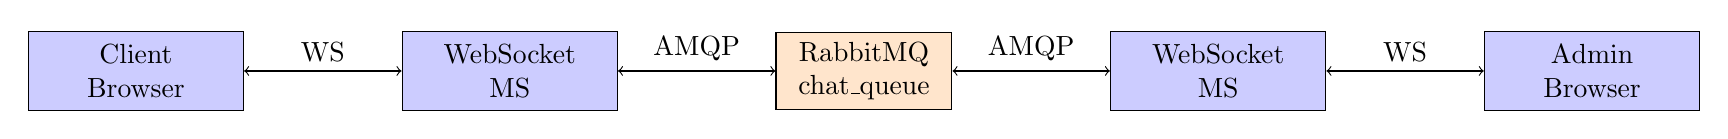
\begin{tikzpicture}[node distance=1.5cm, auto]
    \tikzstyle{box} = [rectangle, draw, fill=blue!20, text width=2.5cm, text centered, minimum height=1cm]
    \tikzstyle{queue} = [rectangle, draw, fill=orange!20, text width=2cm, text centered]
    
    \node[box] (client) {Client\\Browser};
    \node[box, right=2cm of client] (ws1) {WebSocket\\MS};
    \node[queue, right=2cm of ws1] (rabbit) {RabbitMQ\\chat\_queue};
    \node[box, right=2cm of rabbit] (ws2) {WebSocket\\MS};
    \node[box, right=2cm of ws2] (admin) {Admin\\Browser};
    
    \draw[<->] (client) -- node[above] {WS} (ws1);
    \draw[<->] (ws1) -- node[above] {AMQP} (rabbit);
    \draw[<->] (rabbit) -- node[above] {AMQP} (ws2);
    \draw[<->] (ws2) -- node[above] {WS} (admin);
\end{tikzpicture}
\caption{Client-to-Admin Chat Architecture}
\end{figure}

\subsection{WebSocket Handler}
\begin{lstlisting}[language=Java, caption=ChatWebSocketHandler.java]
@Component
public class ChatWebSocketHandler extends TextWebSocketHandler {
    
    private final Map<String, WebSocketSession> userSessions = 
        new ConcurrentHashMap<>();
    private final Map<String, WebSocketSession> adminSessions = 
        new ConcurrentHashMap<>();
    
    @Override
    public void afterConnectionEstablished(WebSocketSession session) {
        String query = session.getUri().getQuery();
        // Parse userId or adminId from query params
        if (query.contains("userId=")) {
            userSessions.put(userId, session);
        } else if (query.contains("adminId=")) {
            adminSessions.put(adminId, session);
        }
    }
    
    public void sendToUser(String userId, ChatMessage message) {
        WebSocketSession session = userSessions.get(userId);
        if (session != null && session.isOpen()) {
            session.sendMessage(new TextMessage(toJson(message)));
        }
    }
    
    public void broadcastToAllAdmins(ChatMessage message) {
        adminSessions.values().forEach(session -> {
            if (session.isOpen()) {
                session.sendMessage(new TextMessage(toJson(message)));
            }
        });
    }
}
\end{lstlisting}

\subsection{Frontend Implementation}

\subsubsection{Client Chat Interface}
\begin{itemize}
    \item Toggle between "Bot Mode" and "Admin Mode"
    \item Bot Mode: Uses rule-based + AI chatbot
    \item Admin Mode: Connects via WebSocket for real-time chat
    \item Shows "Connected to Admin" status indicator
    \item Displays "Waiting for admin response..." when waiting
\end{itemize}

\subsubsection{Admin Chat Interface}
\begin{itemize}
    \item Dedicated page at \texttt{/dashboard/admin-chat}
    \item Sidebar with list of active conversations
    \item Badge showing unread message count
    \item Real-time message updates via WebSocket
    \item Only accessible to users with ADMIN role
\end{itemize}

\subsection{Custom React Hook}
\begin{lstlisting}[language=JavaScript, caption=useWebSocketChat.ts]
export function useWebSocketChat({ userId, isAdmin, enabled }) {
  const [isConnected, setIsConnected] = useState(false);
  const wsRef = useRef<WebSocket | null>(null);
  
  const connect = useCallback(() => {
    if (!enabled) return;
    
    const wsUrl = isAdmin
      ? `ws://localhost:8085/ws/chat?adminId=${userId}`
      : `ws://localhost:8085/ws/chat?userId=${userId}`;
    
    const ws = new WebSocket(wsUrl);
    
    ws.onopen = () => setIsConnected(true);
    ws.onmessage = (event) => {
      const message = JSON.parse(event.data);
      onMessageReceived?.(message);
    };
    ws.onclose = () => setIsConnected(false);
    
    wsRef.current = ws;
  }, [userId, isAdmin, enabled]);
  
  return { isConnected, sendMessage, disconnect };
}
\end{lstlisting}

% ============================================
% SECTION 7: WALL-E MASCOT
% ============================================
\section{Wall-E Mascot Feature}

\subsection{Overview}
A fun interactive mascot (Wall-E robot) was added to the chat interface. The mascot displays a looping video in the bottom-right corner of the AI Support page.

\subsection{Implementation}
\begin{lstlisting}[language=JavaScript, caption=WallEMascot Component]
export function WallEMascot() {
  const videoRef = useRef<HTMLVideoElement>(null);

  return (
    <div className="fixed" style={{ 
      position: 'fixed', 
      bottom: '1rem', 
      right: '1rem', 
      zIndex: 9999,
      width: '200px',
      height: '200px',
      pointerEvents: 'none'
    }}>
      {/* Glow effect */}
      <div className="absolute -inset-2 bg-gradient-to-r 
        from-cyan-500/30 to-purple-500/30 rounded-2xl 
        blur-lg opacity-60" />
      
      {/* Video container */}
      <div className="relative w-full h-full rounded-2xl 
        overflow-hidden border-2 border-cyan-500/40 
        shadow-xl bg-black/20">
        <video
          ref={videoRef}
          className="w-full h-full object-cover"
          muted loop autoPlay playsInline
        >
          <source src="/wall-e.mp4" type="video/mp4" />
        </video>
      </div>
    </div>
  );
}
\end{lstlisting}

\subsection{Features}
\begin{itemize}
    \item Video plays in loop automatically
    \item Non-clickable (pointer-events: none)
    \item Cyan/purple glow effect
    \item Rounded corners with border
    \item Only visible on the AI Support chat page
\end{itemize}

% ============================================
% SECTION 8: DOCKER DEPLOYMENT
% ============================================
\section{Docker Deployment}

\subsection{Docker Compose Services}
\begin{lstlisting}[language=yaml, caption=docker-compose.yml (New Services)]
services:
  websocket-microservice:
    build: ./websocket-microservice
    container_name: websocket-microservice-app
    ports:
      - "8085:8085"
    environment:
      - SPRING_RABBITMQ_HOST=rabbitmq
    depends_on:
      rabbitmq:
        condition: service_healthy
    networks:
      - energy-network
    labels:
      - "traefik.enable=true"
      - "traefik.http.routers.websocket.rule=PathPrefix(`/ws`)"

  customer-support-microservice:
    build: ./customer-support-microservice
    container_name: customer-support-microservice-app
    ports:
      - "8086:8086"
    environment:
      - GEMINI_API_KEY=${GEMINI_API_KEY}
      - SPRING_RABBITMQ_HOST=rabbitmq
    depends_on:
      rabbitmq:
        condition: service_healthy
    networks:
      - energy-network
    labels:
      - "traefik.enable=true"
      - "traefik.http.routers.support.rule=PathPrefix(`/api/chat`)"
\end{lstlisting}

\subsection{Build and Run Commands}
\begin{lstlisting}[language=bash, caption=Deployment Commands]
# Build all services
docker-compose build

# Start all services
docker-compose up -d

# Check status
docker-compose ps

# View logs
docker-compose logs -f websocket-microservice
docker-compose logs -f customer-support-microservice

# Rebuild specific service
docker-compose build --no-cache websocket-microservice
docker-compose up -d websocket-microservice
\end{lstlisting}

% ============================================
% SECTION 9: THEORETICAL QUESTIONS
% ============================================
\section{Theoretical Questions}

\subsection{Load Balancing}

\subsubsection{Definition}
Load balancing is the process of distributing network traffic across multiple servers to ensure no single server bears too much demand. This improves application availability, scalability, and performance.

\subsubsection{Types of Load Balancing}
\begin{table}[H]
\centering
\begin{tabular}{|l|p{8cm}|}
\hline
\textbf{Algorithm} & \textbf{Description} \\
\hline
Round Robin & Distributes requests sequentially to each server \\
\hline
Least Connections & Routes to server with fewest active connections \\
\hline
IP Hash & Routes based on client IP address (session persistence) \\
\hline
Weighted & Distributes based on server capacity/weight \\
\hline
Random & Randomly selects a server \\
\hline
\end{tabular}
\caption{Load Balancing Algorithms}
\end{table}

\subsubsection{Implementation in Assignment 3}
\begin{itemize}
    \item \textbf{Traefik} acts as reverse proxy and load balancer
    \item Routes requests to appropriate microservices
    \item Can scale services with Docker Swarm
    \item Example: Multiple replicas of Monitoring MS
\end{itemize}

\subsection{Docker Swarm}

\subsubsection{Definition}
Docker Swarm is Docker's native container orchestration tool that allows you to manage a cluster of Docker nodes as a single virtual system.

\subsubsection{Key Concepts}
\begin{itemize}
    \item \textbf{Manager Nodes}: Control the cluster, schedule tasks
    \item \textbf{Worker Nodes}: Execute containers
    \item \textbf{Services}: Define applications to run
    \item \textbf{Tasks}: Individual container instances
    \item \textbf{Replicas}: Number of container copies
\end{itemize}

\subsubsection{Commands}
\begin{lstlisting}[language=bash, caption=Docker Swarm Commands]
# Initialize swarm
docker swarm init

# Deploy stack
docker stack deploy -c docker-compose.yml energy-stack

# Scale service
docker service scale energy-stack_monitoring-microservice=3

# List services
docker service ls

# View service logs
docker service logs energy-stack_websocket-microservice
\end{lstlisting}

\subsubsection{Advantages}
\begin{itemize}
    \item \textbf{Auto-healing}: Automatically restarts failed containers
    \item \textbf{Rolling updates}: Update without downtime
    \item \textbf{Load balancing}: Built-in traffic distribution
    \item \textbf{Scaling}: Easy horizontal scaling
\end{itemize}

\subsection{Sockets vs WebSockets}

\subsubsection{Traditional Sockets (TCP/IP)}
\begin{itemize}
    \item Low-level network communication
    \item Bidirectional, persistent connection
    \item Used for: SSH, FTP, database connections
    \item Requires custom protocol implementation
\end{itemize}

\subsubsection{WebSockets}
\begin{itemize}
    \item Protocol built on top of HTTP
    \item Full-duplex communication over single TCP connection
    \item Starts with HTTP handshake, then upgrades to WebSocket
    \item Native browser support via JavaScript API
\end{itemize}

\subsubsection{Comparison}
\begin{table}[H]
\centering
\begin{tabular}{|l|l|l|}
\hline
\textbf{Feature} & \textbf{HTTP} & \textbf{WebSocket} \\
\hline
Connection & Request-Response & Persistent \\
Direction & Unidirectional & Bidirectional \\
Overhead & High (headers each request) & Low (after handshake) \\
Latency & Higher & Lower \\
Use Case & REST APIs, Web pages & Real-time apps, Chat \\
\hline
\end{tabular}
\caption{HTTP vs WebSocket Comparison}
\end{table}

\subsubsection{WebSocket Handshake}
\begin{lstlisting}[caption=WebSocket Handshake Process]
Client Request:
GET /ws/chat HTTP/1.1
Host: localhost:8085
Upgrade: websocket
Connection: Upgrade
Sec-WebSocket-Key: dGhlIHNhbXBsZSBub25jZQ==
Sec-WebSocket-Version: 13

Server Response:
HTTP/1.1 101 Switching Protocols
Upgrade: websocket
Connection: Upgrade
Sec-WebSocket-Accept: s3pPLMBiTxaQ9kYGzzhZRbK+xOo=
\end{lstlisting}

\subsubsection{Implementation in Assignment 3}
\begin{itemize}
    \item \textbf{Endpoint}: \texttt{ws://localhost:8085/ws/notifications}
    \item \textbf{Purpose}: Real-time overconsumption alerts
    \item \textbf{Chat Endpoint}: \texttt{ws://localhost:8085/ws/chat}
    \item \textbf{Purpose}: Bidirectional client-admin chat
\end{itemize}

\subsection{Security in Web Applications}

\subsubsection{Authentication vs Authorization}
\begin{itemize}
    \item \textbf{Authentication}: "Who are you?" - Verifying identity
    \item \textbf{Authorization}: "What can you do?" - Verifying permissions
\end{itemize}

\subsubsection{JWT (JSON Web Token)}
\begin{lstlisting}[caption=JWT Structure]
Header.Payload.Signature

Header: {"alg": "HS256", "typ": "JWT"}
Payload: {"sub": "user123", "role": "ADMIN", "exp": 1234567890}
Signature: HMACSHA256(base64(header) + "." + base64(payload), secret)
\end{lstlisting}

\subsubsection{Security Best Practices}
\begin{enumerate}
    \item \textbf{HTTPS}: Encrypt all communications
    \item \textbf{Password Hashing}: Use BCrypt with salt
    \item \textbf{Input Validation}: Sanitize all user input
    \item \textbf{CORS Configuration}: Restrict allowed origins
    \item \textbf{Rate Limiting}: Prevent brute force attacks
    \item \textbf{SQL Injection Prevention}: Use prepared statements
    \item \textbf{XSS Prevention}: Escape user-generated content
    \item \textbf{CSRF Protection}: Use tokens for state-changing requests
\end{enumerate}

\subsubsection{Security in Assignment 3}
\begin{itemize}
    \item JWT for stateless authentication
    \item BCrypt for password hashing
    \item CORS configured for WebSocket connections
    \item Traefik as security layer (reverse proxy)
    \item Role-based access control (ADMIN vs CLIENT)
    \item WebSocket authentication via query parameters
\end{itemize}

% ============================================
% SECTION 10: TESTING
% ============================================
\section{Testing Guide}

\subsection{Test 1: Overconsumption Alert}
\begin{enumerate}
    \item Create a device with \texttt{maxHourlyConsumption = 5.0} kWh
    \item Configure device simulator with the device ID
    \item Run simulator: \texttt{python device-simulator/simulator.py}
    \item Wait for 6 measurements (60 seconds)
    \item Verify toast notification appears in frontend
    \item Check RabbitMQ queue: \texttt{overconsumption\_queue}
\end{enumerate}

\subsection{Test 2: Rule-Based Chat}
\begin{enumerate}
    \item Open \texttt{http://localhost:3000/dashboard/chat}
    \item Send message: "hello"
    \item Verify response: "Hello! Welcome to Energy Management Support..."
    \item Verify green "Rule" badge appears
    \item Test other keywords: "help", "device", "consumption"
\end{enumerate}

\subsection{Test 3: AI Chat (Bonus)}
\begin{enumerate}
    \item Send a complex question not matching any rule
    \item Example: "What are the best practices for reducing energy waste?"
    \item Verify AI-generated response appears
    \item Verify blue "AI" badge with sparkle icon
    \item Check response is contextually relevant
\end{enumerate}

\subsection{Test 4: Client-to-Admin Chat (Bonus)}
\begin{enumerate}
    \item \textbf{Tab 1 - Client}:
    \begin{itemize}
        \item Login as client user
        \item Go to AI Support page
        \item Click "Admin" toggle button
        \item Verify "Connected to Admin" status
        \item Send message: "Hello admin, I need help!"
    \end{itemize}
    \item \textbf{Tab 2 - Admin}:
    \begin{itemize}
        \item Open incognito/different browser
        \item Login as admin (admin/admin123)
        \item Go to "Admin Chat" in sidebar
        \item Verify "Connected" status
        \item See client's message in conversation list
        \item Click conversation and reply
    \end{itemize}
    \item \textbf{Verify}: Client receives admin's response in real-time
\end{enumerate}

\subsection{Test 5: Wall-E Mascot}
\begin{enumerate}
    \item Navigate to \texttt{/dashboard/chat}
    \item Verify Wall-E video appears in bottom-right corner
    \item Verify video plays in loop
    \item Verify mascot is not clickable
    \item Navigate to other pages - mascot should not appear
\end{enumerate}

% ============================================
% SECTION 11: TROUBLESHOOTING
% ============================================
\section{Troubleshooting}

\subsection{WebSocket Connection Failed}
\begin{itemize}
    \item Verify WebSocket MS is running: \texttt{docker ps | grep websocket}
    \item Check logs: \texttt{docker logs websocket-microservice-app}
    \item Verify CORS settings in WebSocketConfig.java
    \item Check browser console for connection errors
    \item Ensure port 8085 is not blocked by firewall
\end{itemize}

\subsection{Chat Not Responding}
\begin{itemize}
    \item Check Customer Support MS logs
    \item Verify rules are loaded: \texttt{GET /api/chat/rules}
    \item For AI responses, verify Gemini API key is valid
    \item Check RabbitMQ connection for admin chat
\end{itemize}

\subsection{Notifications Not Appearing}
\begin{itemize}
    \item Verify RabbitMQ queue exists: \texttt{overconsumption\_queue}
    \item Check Monitoring MS detects overconsumption
    \item Verify WebSocket connection in browser console
    \item Check WebSocket MS logs for broadcast messages
\end{itemize}

\subsection{Docker Build Failures}
\begin{itemize}
    \item Clear Docker cache: \texttt{docker system prune -a}
    \item Rebuild without cache: \texttt{docker-compose build --no-cache}
    \item Check Dockerfile syntax
    \item Verify all dependencies in pom.xml
\end{itemize}

% ============================================
% SECTION 12: DEPLOYMENT DIAGRAM
% ============================================
\section{Deployment Diagram}

\subsection{System Components}
\begin{figure}[H]
\centering
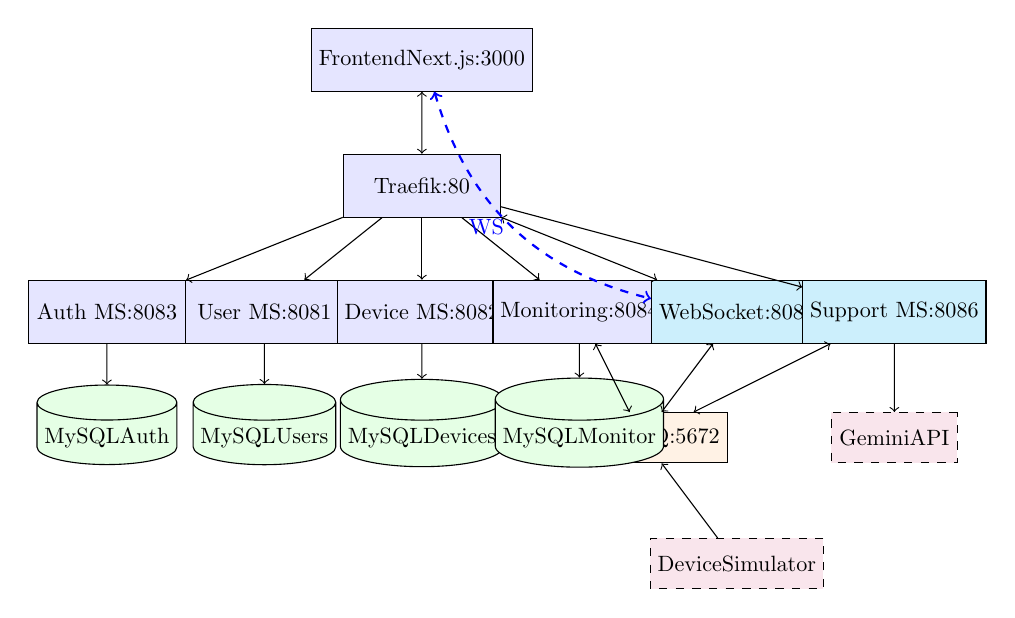
\begin{tikzpicture}[scale=0.8, transform shape]
    % Styles
    \tikzstyle{container} = [rectangle, draw, fill=blue!10, minimum width=2.5cm, minimum height=1cm, text centered]
    \tikzstyle{database} = [cylinder, draw, fill=green!10, shape border rotate=90, aspect=0.25, minimum height=1cm, minimum width=1.5cm]
    \tikzstyle{queue} = [rectangle, draw, fill=orange!10, minimum width=2cm, minimum height=0.8cm]
    \tikzstyle{external} = [rectangle, draw, fill=purple!10, minimum width=2cm, minimum height=0.8cm, dashed]
    
    % Frontend
    \node[container] (frontend) at (0,6) {Frontend\\Next.js:3000};
    
    % Traefik
    \node[container] (traefik) at (0,4) {Traefik\\:80};
    
    % Microservices Row 1
    \node[container] (auth) at (-5,2) {Auth MS\\:8083};
    \node[container] (user) at (-2.5,2) {User MS\\:8081};
    \node[container] (device) at (0,2) {Device MS\\:8082};
    \node[container] (monitoring) at (2.5,2) {Monitoring\\:8084};
    \node[container, fill=cyan!20] (websocket) at (5,2) {WebSocket\\:8085};
    
    % Customer Support
    \node[container, fill=cyan!20] (support) at (7.5,2) {Support MS\\:8086};
    
    % RabbitMQ
    \node[queue] (rabbitmq) at (3.5,0) {RabbitMQ\\:5672};
    
    % Databases
    \node[database] (db1) at (-5,0) {MySQL\\Auth};
    \node[database] (db2) at (-2.5,0) {MySQL\\Users};
    \node[database] (db3) at (0,0) {MySQL\\Devices};
    \node[database] (db4) at (2.5,0) {MySQL\\Monitor};
    
    % External
    \node[external] (gemini) at (7.5,0) {Gemini\\API};
    \node[external] (simulator) at (5,-2) {Device\\Simulator};
    
    % Connections
    \draw[<->] (frontend) -- (traefik);
    \draw[->] (traefik) -- (auth);
    \draw[->] (traefik) -- (user);
    \draw[->] (traefik) -- (device);
    \draw[->] (traefik) -- (monitoring);
    \draw[<->] (traefik) -- (websocket);
    \draw[->] (traefik) -- (support);
    
    \draw[->] (auth) -- (db1);
    \draw[->] (user) -- (db2);
    \draw[->] (device) -- (db3);
    \draw[->] (monitoring) -- (db4);
    
    \draw[<->] (monitoring) -- (rabbitmq);
    \draw[<->] (websocket) -- (rabbitmq);
    \draw[<->] (support) -- (rabbitmq);
    \draw[->] (simulator) -- (rabbitmq);
    
    \draw[->] (support) -- (gemini);
    
    % WebSocket direct connection
    \draw[<->, dashed, thick, blue] (frontend) to[bend right=30] node[left] {WS} (websocket);
\end{tikzpicture}
\caption{Complete System Deployment Diagram}
\end{figure}

\subsection{Network Configuration}
\begin{table}[H]
\centering
\begin{tabular}{|l|l|l|}
\hline
\textbf{Service} & \textbf{Internal Port} & \textbf{External Port} \\
\hline
Frontend & 3000 & 3000 \\
Traefik & 80 & 80 \\
Auth MS & 8083 & - (via Traefik) \\
User MS & 8081 & - (via Traefik) \\
Device MS & 8082 & - (via Traefik) \\
Monitoring MS & 8084 & - (via Traefik) \\
WebSocket MS & 8085 & 8085 \\
Customer Support MS & 8086 & 8086 \\
RabbitMQ & 5672 & 5672 \\
RabbitMQ Management & 15672 & 15672 \\
MySQL Auth & 3306 & 3309 \\
MySQL Users & 3306 & 3307 \\
MySQL Devices & 3306 & 3308 \\
MySQL Monitoring & 3306 & 3310 \\
\hline
\end{tabular}
\caption{Port Configuration}
\end{table}

% ============================================
% SECTION 13: QUICK START GUIDE
% ============================================
\section{Quick Start Guide}

\subsection{Prerequisites}
\begin{itemize}
    \item Docker \& Docker Compose installed
    \item Python 3.x (for device simulator)
    \item Google Gemini API Key (for AI support - bonus)
    \item Git (for cloning repository)
\end{itemize}

\subsection{Installation Steps}
\begin{lstlisting}[language=bash, caption=Installation Commands]
# 1. Clone repository
git clone <repository-url>
cd energy-management-system

# 2. Set environment variables (optional for AI)
export GEMINI_API_KEY=your-api-key-here

# 3. Build all services
docker-compose build

# 4. Start all services
docker-compose up -d

# 5. Verify services are running
docker-compose ps

# 6. Check logs
docker-compose logs -f
\end{lstlisting}

\subsection{Access Points}
\begin{table}[H]
\centering
\begin{tabular}{|l|l|}
\hline
\textbf{Service} & \textbf{URL} \\
\hline
Frontend & http://localhost:3000 \\
Traefik Dashboard & http://localhost:8080 \\
RabbitMQ Management & http://localhost:15672 \\
WebSocket Notifications & ws://localhost:8085/ws/notifications \\
WebSocket Chat & ws://localhost:8085/ws/chat \\
Chat API & http://localhost/api/chat \\
\hline
\end{tabular}
\caption{Service Access URLs}
\end{table}

\subsection{Default Credentials}
\begin{table}[H]
\centering
\begin{tabular}{|l|l|l|}
\hline
\textbf{Service} & \textbf{Username} & \textbf{Password} \\
\hline
RabbitMQ & guest & guest \\
Admin User & admin & admin123 \\
Client User & (create via registration) & - \\
\hline
\end{tabular}
\caption{Default Credentials}
\end{table}

% ============================================
% SECTION 14: SCORING SUMMARY
% ============================================
\section{Scoring Summary}

\begin{table}[H]
\centering
\begin{tabular}{|l|l|l|l|}
\hline
\textbf{Phase} & \textbf{Description} & \textbf{Points} & \textbf{Status} \\
\hline
Phase 1 & WebSocket MS + Overconsumption Alerts & 2.5p & \checkmark Completed \\
Phase 2 & Rule-Based Chatbot (11 rules) & 2.5p & \checkmark Completed \\
Phase 3 & AI-Driven Support (Gemini API) & +1p (Bonus) & \checkmark Completed \\
Phase 4 & Client-to-Admin Chat & +2p (Bonus) & \checkmark Completed \\
Phase 5 & Documentation \& Deployment & - & \checkmark Completed \\
\hline
\multicolumn{2}{|l|}{\textbf{Total}} & \textbf{8p} & \textbf{100\%} \\
\hline
\end{tabular}
\caption{Assignment 3 Scoring}
\end{table}

\subsection{Features Implemented}
\begin{itemize}
    \item[$\checkmark$] WebSocket Microservice with real-time notifications
    \item[$\checkmark$] RabbitMQ integration for message queuing
    \item[$\checkmark$] Overconsumption detection and alerts
    \item[$\checkmark$] Rule-based chatbot with 11 rules
    \item[$\checkmark$] Google Gemini AI integration
    \item[$\checkmark$] Client-to-Admin bidirectional chat
    \item[$\checkmark$] Wall-E mascot on chat page
    \item[$\checkmark$] Docker containerization
    \item[$\checkmark$] Traefik reverse proxy
    \item[$\checkmark$] Complete documentation
\end{itemize}
